\section*{Dissertation Structure}

\begin{frame}[t]
    \sectionpage\vfill
    \begin{figure}
        \centering
        \begin{tikzpicture}
            \visible<1>{\node[inner sep=0pt] (russell) at (0,0) {
\includegraphics[width=.9\textwidth]{graphics/dissertationgraph-0.pdf}};}
            \visible<2>{\node[inner sep=0pt] (russell) at (0,0) {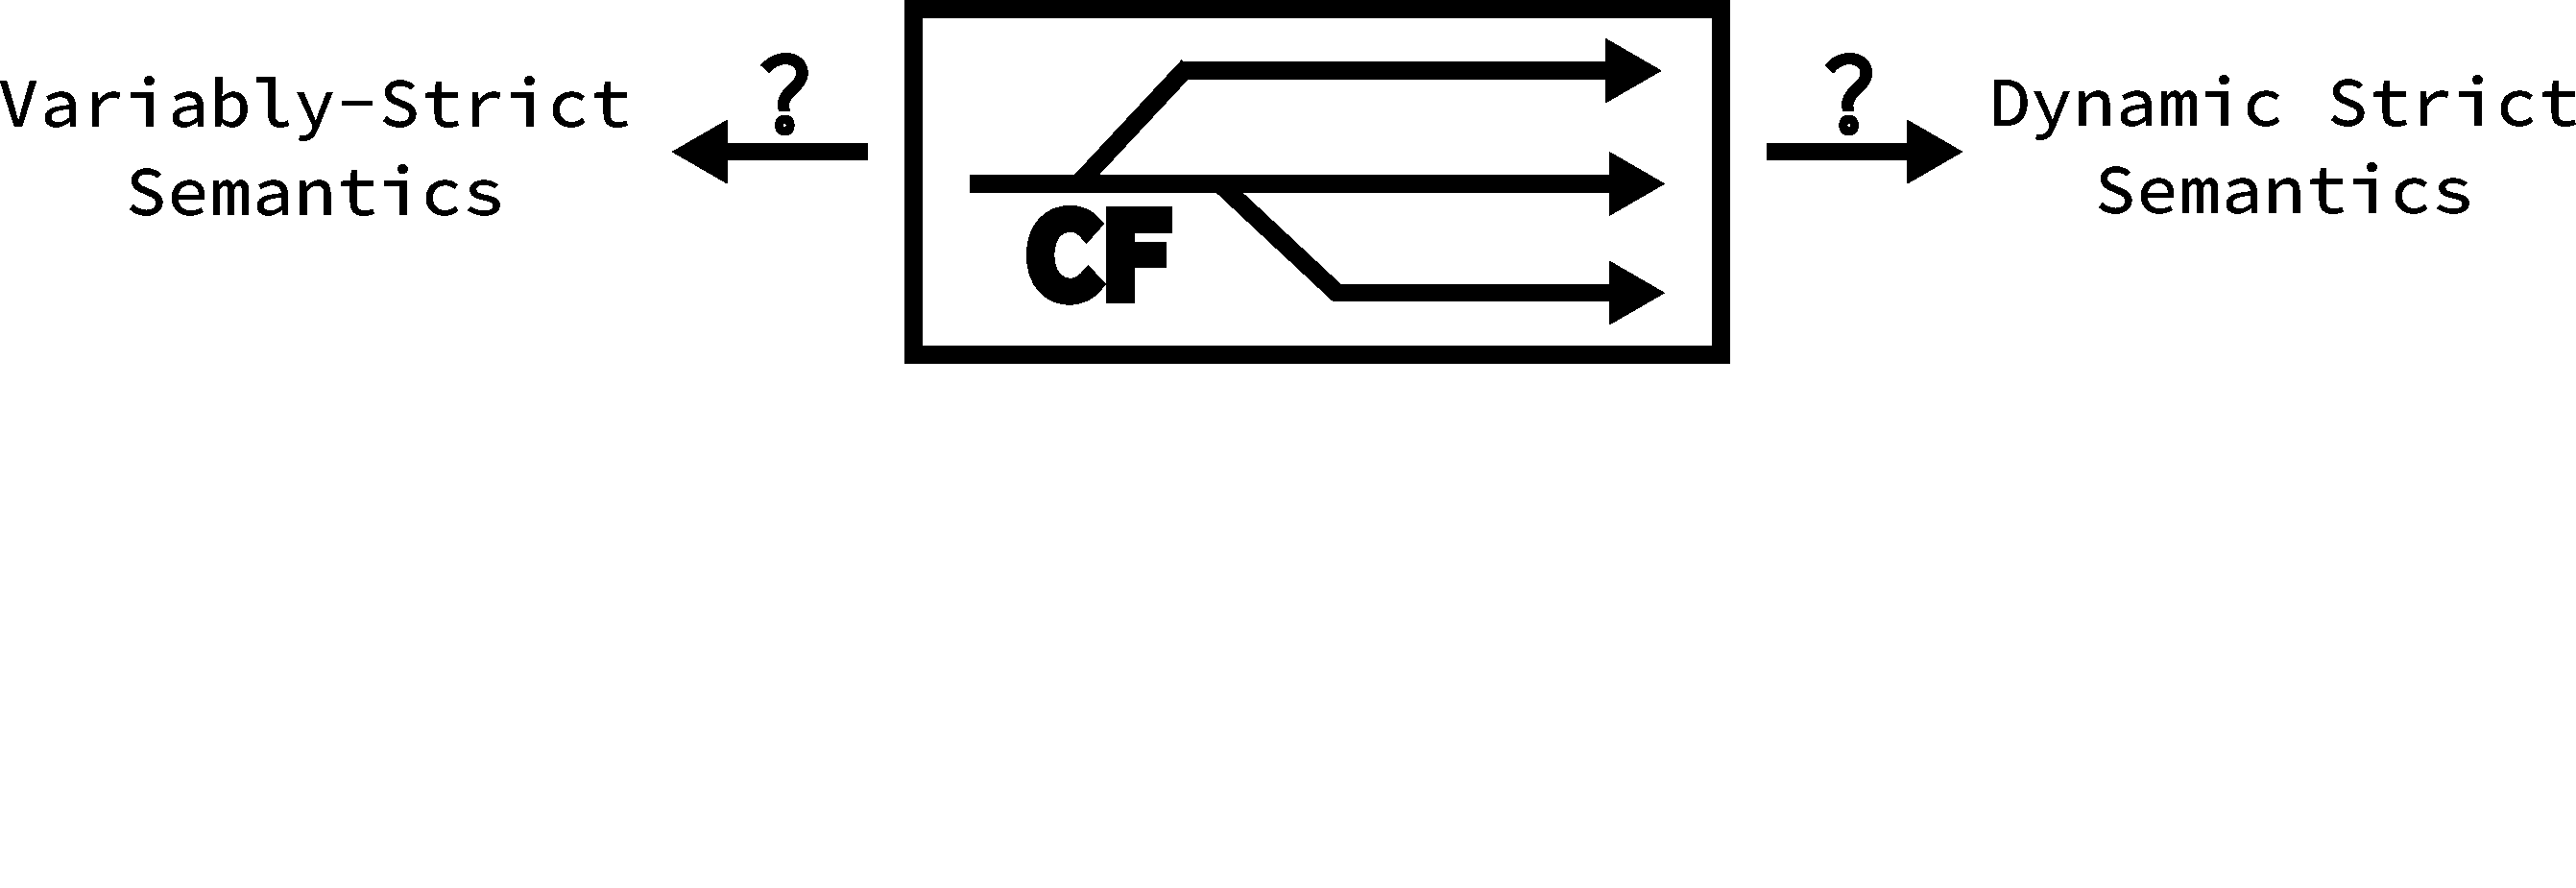
\includegraphics[width=.9\textwidth]{graphics/dissertationgraph-1.pdf}};}
            \visible<3>{\node[inner sep=0pt] (russell) at (0,0) {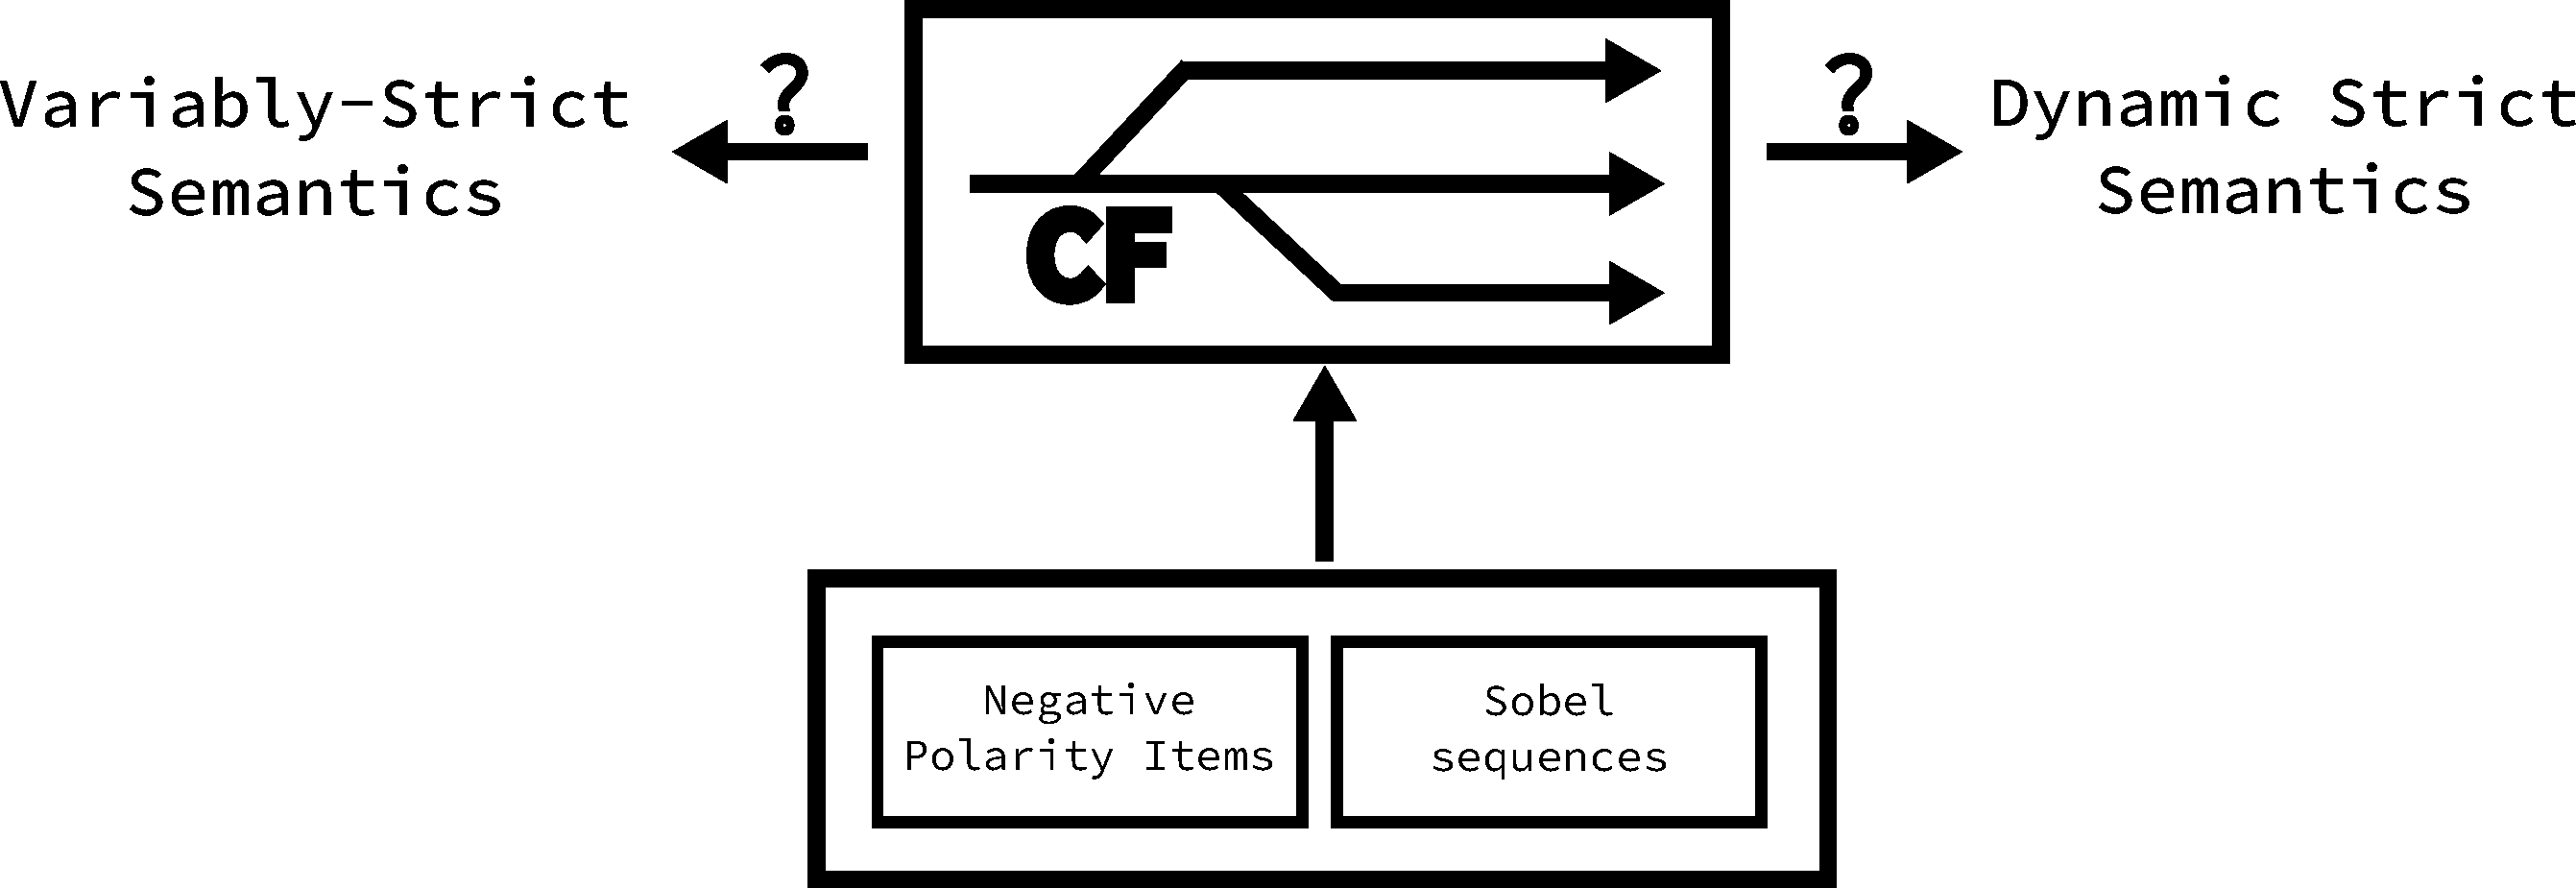
\includegraphics[width=.9\textwidth]{graphics/dissertationgraph-2.pdf}};}
            \visible<4>{\node[inner sep=0pt] (russell) at (0,0) {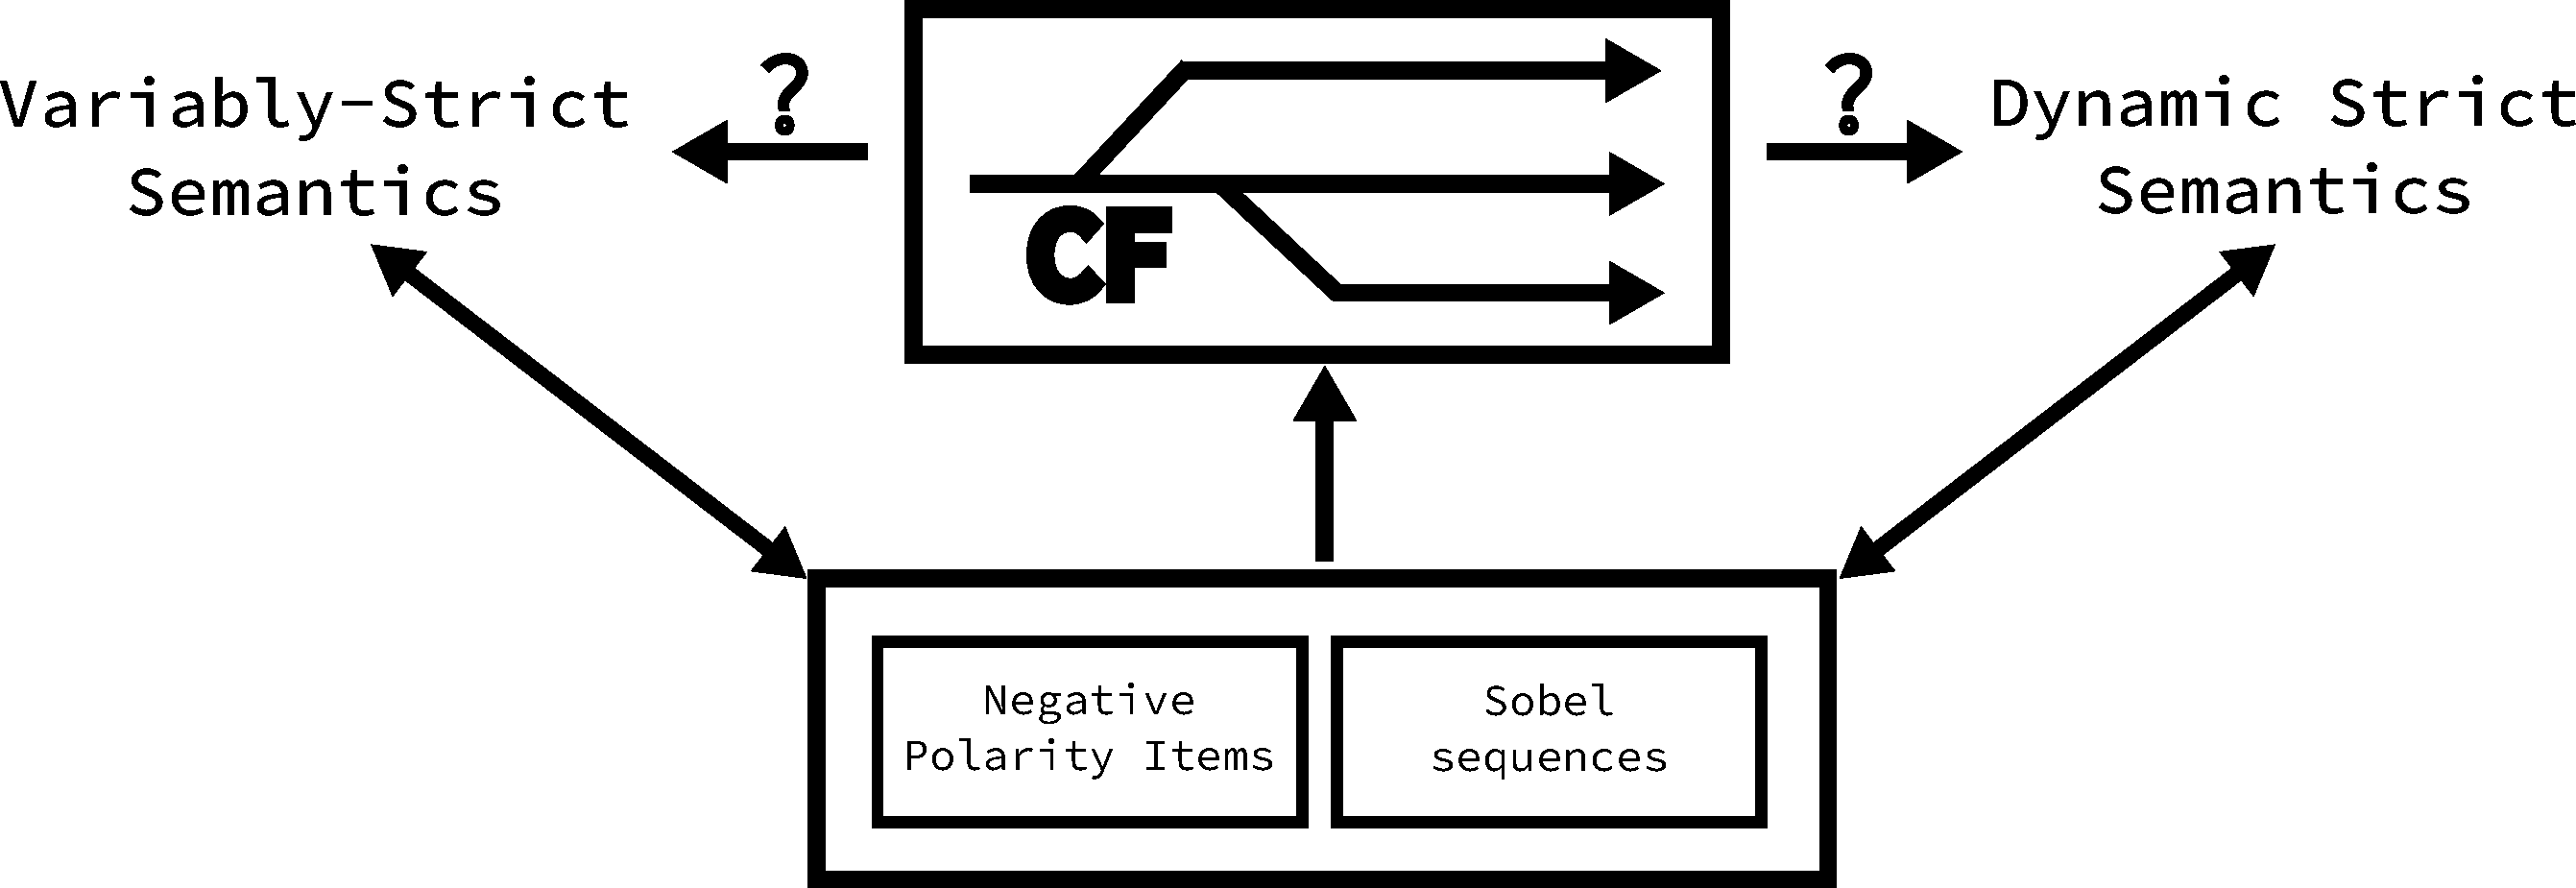
\includegraphics[width=.9\textwidth]{graphics/dissertationgraph-3.pdf}};}
        \end{tikzpicture}
    \end{figure}
    \vfill
\end{frame}

\begin{frame}[t]
	\sectionpage\vskip 9pt
	\begin{itemize}
	    %
		\item[$\blacksquare$]	\textbf{Chapter 2: Negative Polarity Items}\vskip 4.5pt
            \begin{itemize}
                \item<2-> Monotonicity-based approach vs \textit{even}-based approach\vskip 4.5pt
                \item<2-> \textit{Even-Based approach}: solved issue of negative polar question bias\vskip 4.5pt
                \item<2-> \textit{Even-Based approach}; better explanatory power for weak NPIs\vskip 9pt
            \end{itemize}
        \item[$\blacksquare$]	\textbf{Chapter 3: Negative Polarity Items in Conditional Antecedents}\vskip 4.5pt
            \begin{itemize}
                \item<3-> NPI distribution in conditional antecedents\vskip 4.5pt
                \item<3-> Interaction between \textit{even}-based approach and conditional semantics\vskip 4.5pt
                \item<3-> Dynamic strict Approach slightly superior to variably-strict approach
            \end{itemize}
	\end{itemize}
\end{frame}

\begin{frame}[t]
	\sectionpage\vskip 9pt
	\begin{itemize}
        \item[$\blacksquare$]	{\color<5->{seeblau100}\textbf{Chapter 4: Sobel Sequences -- Background and Empirical Data}}\vskip 4.5pt
            \begin{itemize}
                \item<2-> Established felicity distribution of reverse sequences (incl. via an experiment)\vskip 4.5pt
                \item<2-> Isolated felicity factors\vskip 9pt
            \end{itemize}
        \item[$\blacksquare$]	{\color<5->{seeblau100}\textbf{Chapter 5: A Contrast-Based Model of Reverse Sobel Sequence (In)Felicity}}\vskip 4.5pt
            \begin{itemize}
                \item<3-> Implemented model to derive felicity distribution of (reverse) Sobel sequences\vskip 4.5pt
                \item<3-> Showed its interaction with different conditional semantics\vskip 9pt
            \end{itemize}
        \item[$\blacksquare$]	\textbf{Chapter 6: Comparison of Our Model With Ippolito (2020)}\vskip 4.5pt
            \begin{itemize}
                \item<4-> Showed our model better accounts for known data\vskip 4.5pt
                \item<4-> Both models can be reconciled
            \end{itemize}
	\end{itemize}
\end{frame}